\chapter{Fundamentals of the Riemann Pump}
\label{ch:fundamentals}
%\textit{Presentation of the theoretical basis required for an understanding of your work. Do not begin with Newton's laws or Maxwell's equations: imagine that the reader is a competent engineering professor, but not necessarily in your field of expertise. Do not bother to discuss any theory that you do not employ in later sections.}
For the purpose to place this work into the context of the next generation of mobile communication, the concept of software-defined radio is described.
Implemented in this concept, the function, the benefit and some fundamentals of the Riemann Pump are described. 
A demonstrated system shows the \gls{ab:sdr} concept, which is based on the idea to bring the digital domain as close as possible to the antenna.
The Riemann Pump is an arbitrary waveform generator which is controlled by a digital input signal, making it also a custom \gls{ab:dac}.
The concept of the custom designed \gls{ab:dac} as well as some characteristics are presented.
A concise discussion conclude the presented fundamentals.

% Because the analog output signal should be transmitted via an antenna, it has to be enough output power.
%The number of bits, hence the resolution of the \gls{ab:dac} is less stringent as the digital to analog conversion do not distinguish so much within the digital code.
% A crucial point to increase the performance is the oversampling ratio. 
% As the analog signal could consist with some concurrent signals, linearity is crucial to avoid unwanted distortions.
%All these requirements built in one \gls{ab:dac} is not realistic.
%Therefore, intermediate systems have been developed in which the transmitter signal is built by a DAC at lower frequencies, and then up converted with RFFE mostly composed by a linear mixer with a linear PA.
\section{Basic concept of software-defined radio for 5G mobile communication}
The ultimate software defined radio architecture is shown in Figure \ref{fig:ultimateSDR}.
In this vision the analog received signal is directly converted into the digital domain and afterwards filtered, mixed, demodulated and processed.
The absence of the \gls{ab:rffe} is a dream still to come true \cite{RivetDevalJ.-B.EtAl2010}.

\begin{figure}[ht]
	\centering
  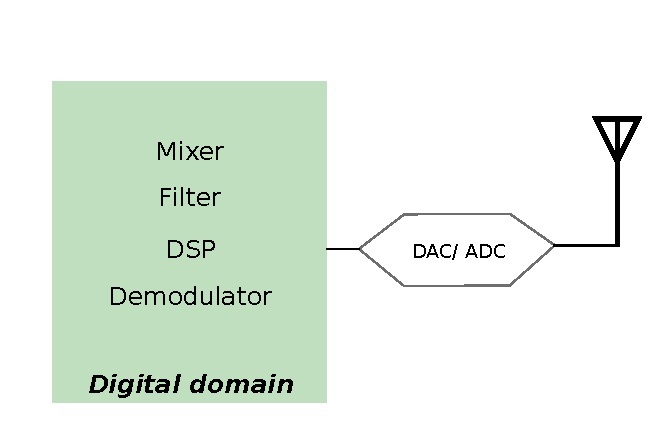
\includegraphics[width=.5\textwidth]{ultimateSDR.pdf}
	\caption{Ultimate Software-defined radio architecture \cite{DevalRivetVeyracEtAl2013}}
	\label{fig:ultimateSDR}
\end{figure}

As Figure \ref{fig:feas_energy} already suggests this is not a realistic option.
The analog components like LNA,filter, mixer have to be implemented separate in the analog domain for the receiving path.
As the transmitter concept is little bit easier

\begin{figure}[htbp]
	% minipage mit (Blind-)Text
	\begin{minipage}{0.49\linewidth} 
	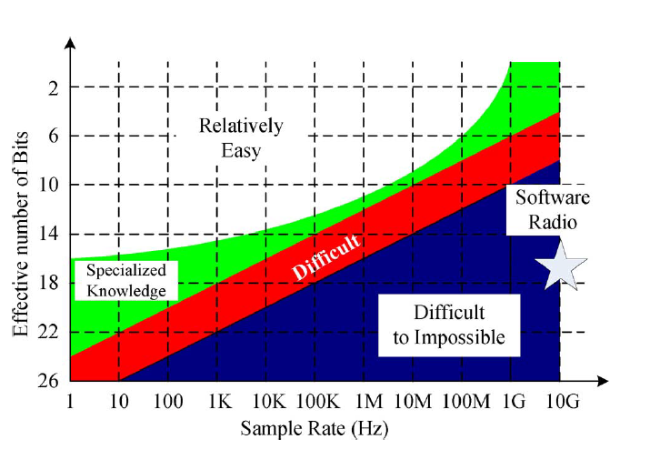
\includegraphics[width=1.1\textwidth]{energy_consumption_sdr.pdf}
	%\caption{Feasibility of Software Radio}
	%\label{energy1} 
	\end{minipage}
	% Auffüllen des Zwischenraums
	\hfill
	% minipage mit Grafik
	\begin{minipage}{0.49\linewidth}
	% \textwidth bezieht sich nun auf die Minipage
	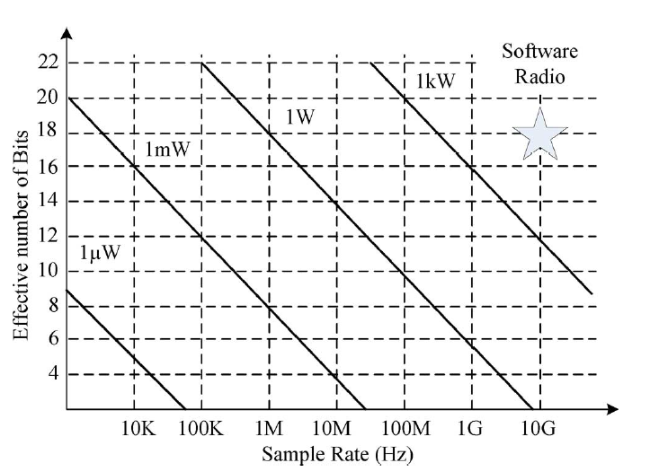
\includegraphics[width=1.1\textwidth]{energy_consumption_sdr2.pdf}
	%\caption{Estimated energy consumption}
	%\label{energy2} 
	\end{minipage}
 \caption{Feasibility (left) and estimation of energy consumption (right) regarding Effective number of Bits and Sample Rate \cite{RivetDevalJ.-B.EtAl2010}}
 \label{fig:feas_energy}
\end{figure}



\section{System design using the Riemann Pump} % PLL and Energy consumption
The focus in this thesis was on the transmitting path of the mentioned system, since the receiving architecture and concepts need a separate investigation.
Further details on the receiving concepts and investigations can be found in \citep{RivetFadhuileDevalEtAl2013}, \cite{RivetDevalD.2008}, \cite{RivetF.2014}, \cite{RivetDevalBegueretJ.-B.2007}.
Focussing on the transmitting path the demand of a \gls{ab:dac} became visible as the digital data must be converted to the analog signal before transmission via the antenna.
As mentioned before high demands are made to the \gls{ab:dac} implemented in a \gls{ab:sdr} concept.\\
One very important requirement is to keep the energy consumption in a moderate range.
If the consumed energy is in the range of several \si{\kilo \watt} it is clear that this is unworkable.
In order to meet \gls{ab:rf} standards the \gls{ab:snr} has to fulfil the limits.
To achieve a moderate \gls{ab:snr} the resolution and the \gls{ab:osr} of the \gls{ab:dac} have to be tuned.
Another crucial aspect is the linearity of the system to avoid unwanted distortions in the propagated signals.
The generated analog output signal, which can consist of a few concurrent signals, has to be amplified for the propagation.\\
The concept of software-defined radio is treated to overcome old problems of mobile communication and hence deal with a fast adapting system which can handle several mobile communication standards at once.
New standards can handled since the system can be changed with an firmware update. 
Therefore every signal within the proposed bandwidth could be processed without changing the hardware, which made it software defined.
The ability to process a spectrum of \gls{ab:dc} to \SI{6}{\giga \hertz} enables it to deal with future mobile communication standards, e.g. IEEE802.11ac (\gls{ab:wlan}) and \gls{ab:lte} already work at \SI{5}{\giga \hertz} and \SI{0.7} ... \SI{2.6}{\giga \hertz}, respectively.\\
To achieve this goal it is essential to bring the digital domain as close as possible to the antenna \cite{RivetDevalBegueretJ.-B.2007}, \cite{DevalRivetVeyracEtAl2013},\cite{RivetDevalJ.-B.EtAl2010}.
The digital domain has a lot of advantages regarding complexity, cost, filtering and processing speed \cite{Grossman2005}.
The structure of digital components is less complex and therefore has less cost.
Digital filtering is more precisely and data processing is more efficient and faster \cite{Chamberlain2015}, \cite{LiRaghunathanJha2009}.\\
% Therefore there is no intermediate step of signal processing which decrease the latency.
%The benefit of this concept is to realize this \gls{ab:dac} as close as possible to the RF front end without an intermediate step of analog signal processing.
% The main drawback of this approach is the energy consumption based on an inefficient ADC/DAC.
%Based on this concept a digital-analog converter is designed to deal with a higher bandwidth than other devices nowadays.
Figure \ref{fig:System} demonstrates the transmitting path of the system design for the concept of \gls{ab:sdr} with the implementation of the Riemann Pump.

\begin{figure}[ht]
	\centering
  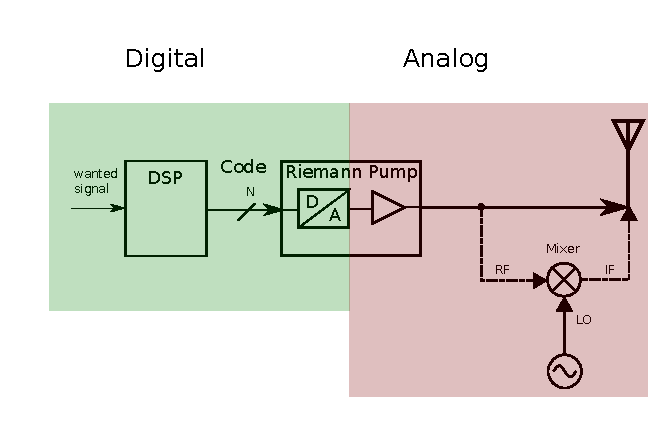
\includegraphics{SystemDesign.pdf}
	\caption{Concept of the Software-defined radio}
	\label{fig:System}
\end{figure}

The demonstrated path in Figure \ref{fig:System} is subdivided into a digital and analog part.
The green digital part is responsible for the calculation of the desired signals and the generation of the corresponding digital code.
A theoretical wanted signal in the time domain, consisting of multiple modulated signals, is fed to a \gls{ab:dsp} which computes a digital bit-stream.
The so called Riemann Code controls the input of a custom \gls{ab:dac}, called Riemann Pump, which is the interface between the digital and the analog part.\\
In the red analog domain the desired signal is amplified by the implemented power transistor in the Riemann Pump and then propagated via the antenna.
Optionally a mixer can be connected to mix the desired signal to even higher frequencies of several tenth of \si{\giga \hertz}.\\
Beside the advantages of the concept there are some constraints on the energy consumption as well as on the real time emission.
Energy consumption is increasing linear with the switching frequency and therefore with the signal bandwidth.
Secondly the real time emission is constrained due to the calculation and conversion of the Riemann Code.

\section{Idea of the Riemann Pump}
\label{IdeaRiemannPump}
Demonstrated the implementation of the Riemann Pump in a system design, the concept of the Riemann Pump itself is presented.\\
Basically the inputs are switches and the output is a capacitance.
The output capacitance (\gls{sy:Cout}) can take any value between the positive (\gls{sy:Vdd}) and negative (\gls{sy:Vss}) power supply voltage by controlling the input switches.\\
This concept is implemented in conventional \glspl{ab:pll} and is known as a charge pump, which is the basic principle of the Riemann Pump \cite{DevalRivetVeyracEtAl2013}, \cite{VeyracRivetDevalEtAl2014}, \cite{DevalRivetVeyrac2015}.
 The integration of electrical current (\gls{sy:iout}) at the capacitance (\gls{sy:Cout}) to form the output voltage  (\gls{sy:Vout}), recalls the founder of the integration principle, Bernhard Riemann.
This integration and the concept of the charge pump lead to the name Riemann Pump, first mentioned 2013 in \cite{DevalRivetVeyracEtAl2013}. \\
Figure \ref{fig:ChargePump} shows the basic principle of a charge pump, used for the digital to analog conversion in this thesis.

\begin{figure}[ht]
	\centering
  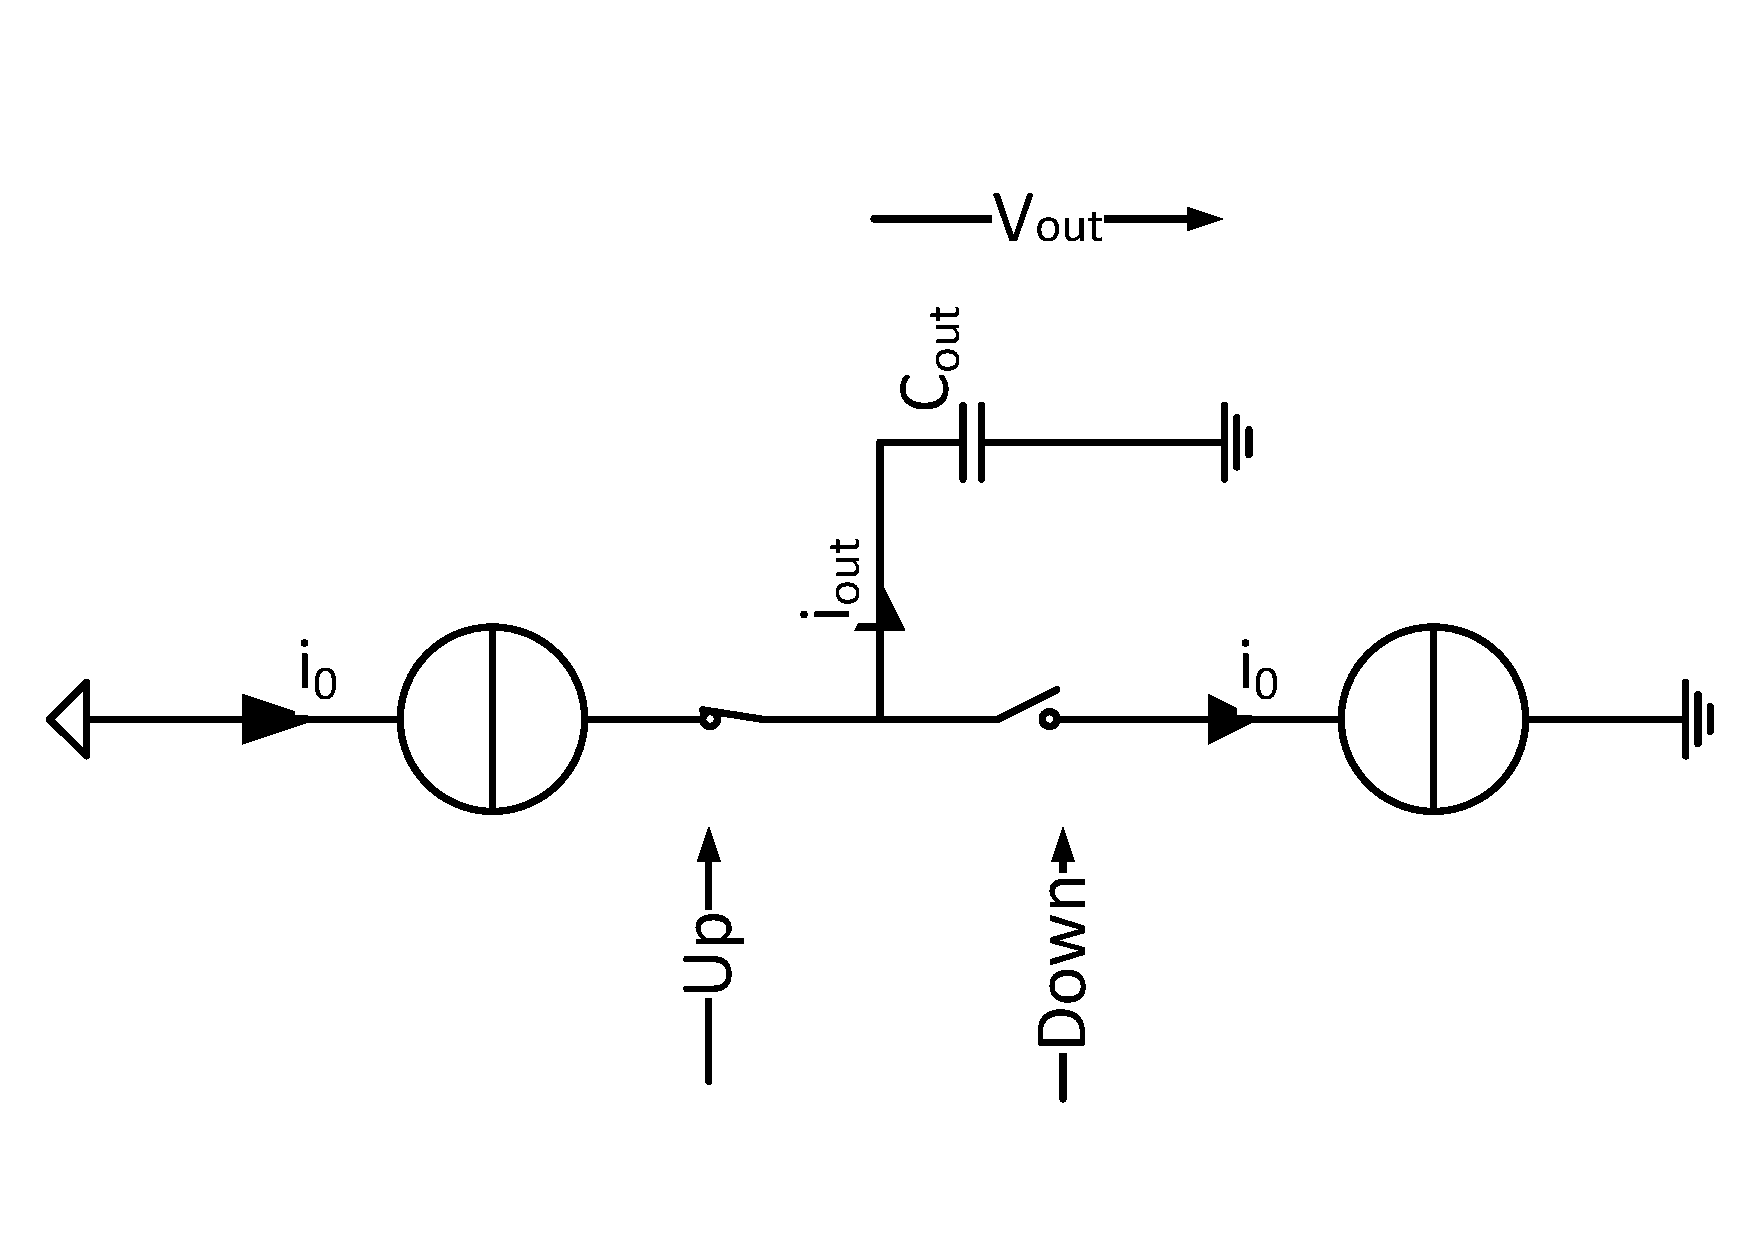
\includegraphics[width=0.5\textwidth, angle = 270]{ChargePump.pdf}
	\caption{scheme of a charge pump}
	\label{fig:ChargePump}
\end{figure}

Increasing the output voltage lead to close the upper switch, also called high side switch, since it switches to the high power potential.
Synchronously the low side switch opens.
Connecting the high side power supply to the capacitor pumps charges onto it forming a voltage over time.
This effect only takes place if the low side switch synchronously opens.
Otherwise the potential at the capacitor is floating and the charge or discharge process is undefined.
Hence these two switches must be controlled with a differential input signal.
For decreasing the output voltage the low side switch has to be closed, while the high side switch is open, to allow the capacitor to discharge.\\
Corresponding to the described principle the output voltage is calculated with 
\begin{equation}
	V_{out} = \frac{1}{C_{out}}{ \int_0^T \! i_{out}(t) \, \mathrm{d}t}.
\end{equation} %%, \hspace{1cm} T = \frac{2*OSR}{f_{sample}

Since the output voltage, consisting of the desired signals, should be propagated via an antenna, the output capacitance can be interpreted as the input stage of a linear power amplifier. 
This input stage consists of a power transistor, which do have the capacitive input impedance characteristic.
The capacitive input characteristic of the connected power transistor enables the system to work without a separate power amplifier.
Implemented in one component this concept saves area and costs and the amplified signal at the drain can be transmitted via the antenna.

%% 20.04 19:00 Uhr

The Riemann Pump is a digital-to-analog converter based on the concept of a charge pump. A few charge pumps with different sized sources in parallel shows the concept of this fast digital to analog converter. With the ability to control the switches really fast, because of the use of GaN25 technology, which have a high transition frequency, a high bandwidth is reached.

\begin{figure}[ht]
	\centering
  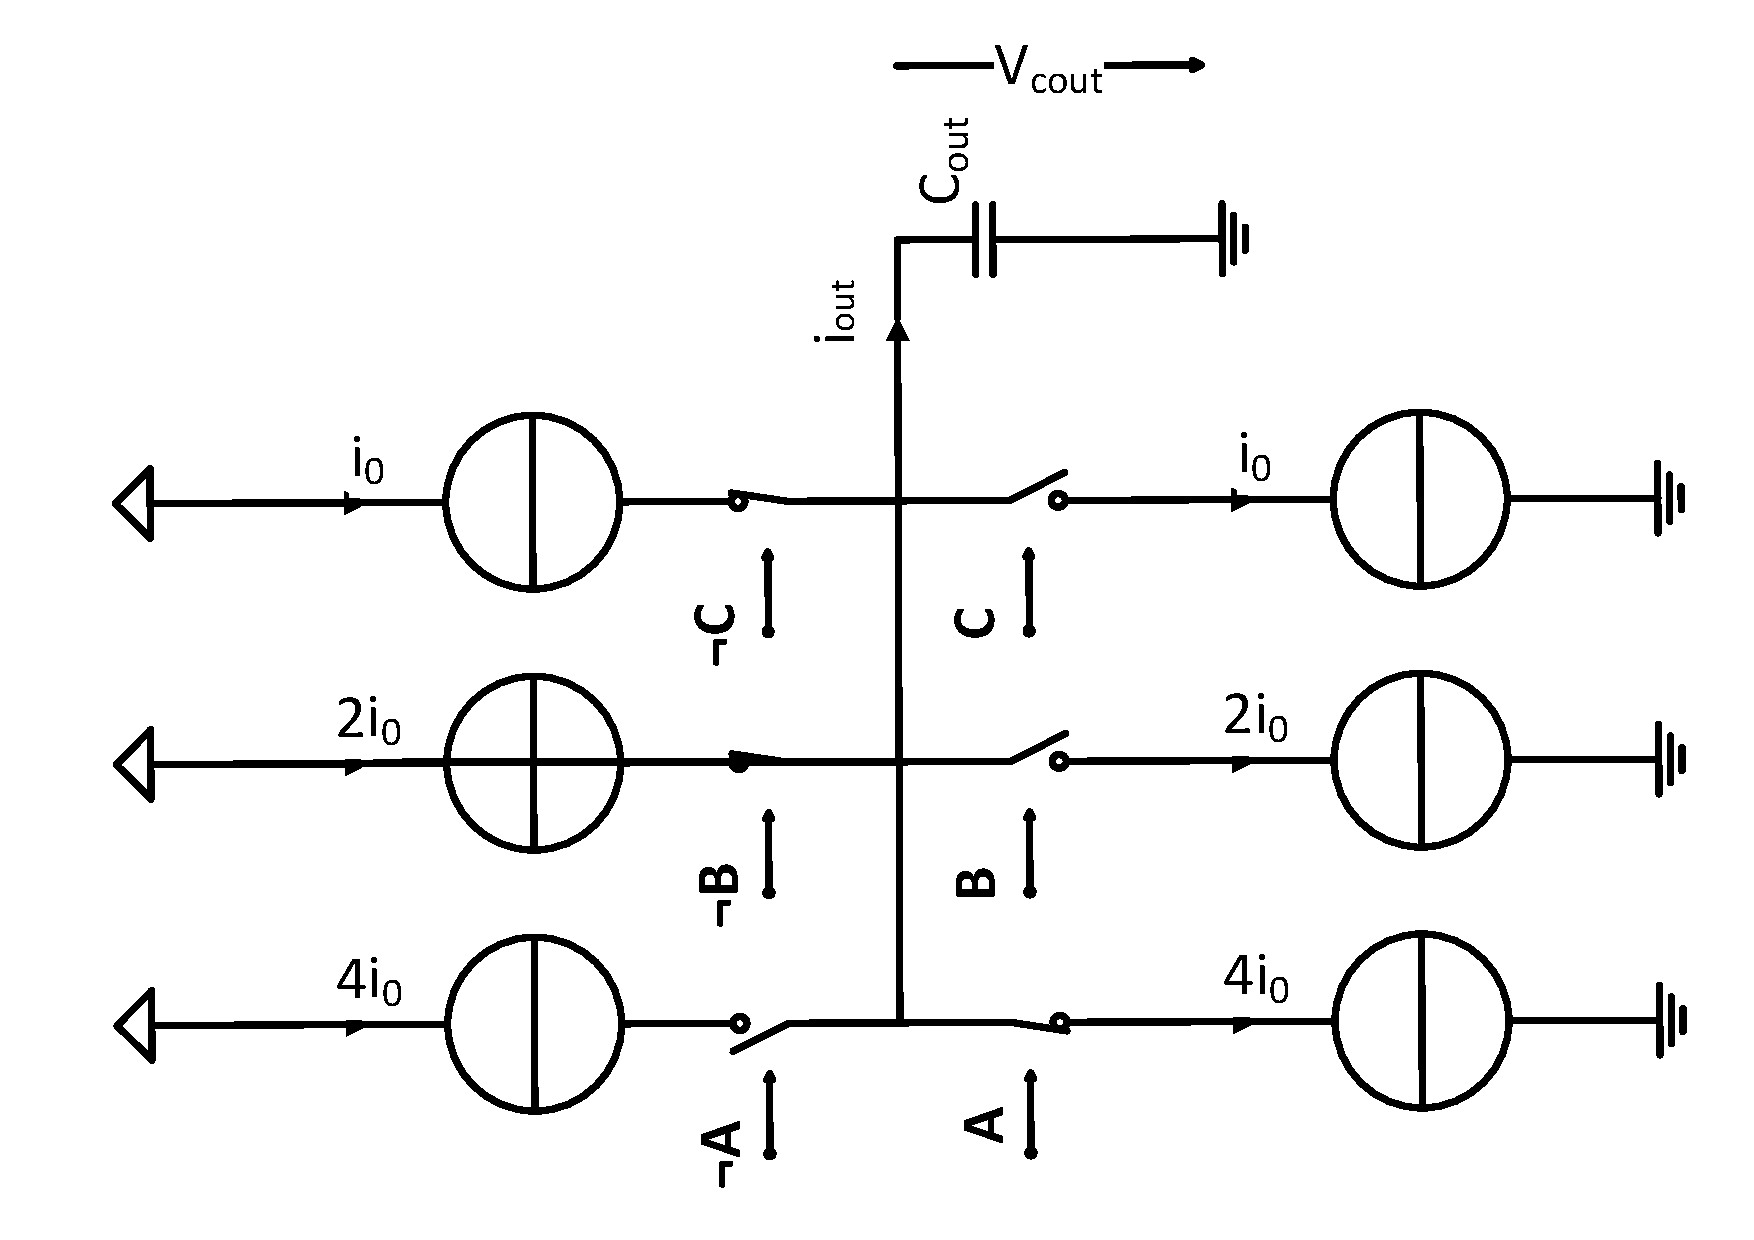
\includegraphics[width=0.5\textwidth, angle = 270]{RP_concept.pdf}
	\caption{Concept of the Riemann Pump with three-bit resolution}
	\label{fig:RiemannPumpConcept}
\end{figure}

 The working principle is to integrate a current into a capacitive load, this integration is based on Riemann Integral, where the name come from. This integration converts the current into a voltage. This output voltage can be applied to the input of a power amp and then to the antenna to propagate it. The current, which charges the capacitive input impedance of the power amp, is controlled by a digital code. A fixed set of slopes, represents the different current sources. A desired signal in the time-domain is generated with MatLab. This signal can consist of many different signals (different carriers and modulation types). This signal is sampled with the given set of slopes. The minimization of the error leads to the Riemann Code. With this Riemann Code (digital) the driver circuit is controlled. This leads to an analog signal formed by the digital input signal. 
 
\begin{figure}[ht]
	\centering
  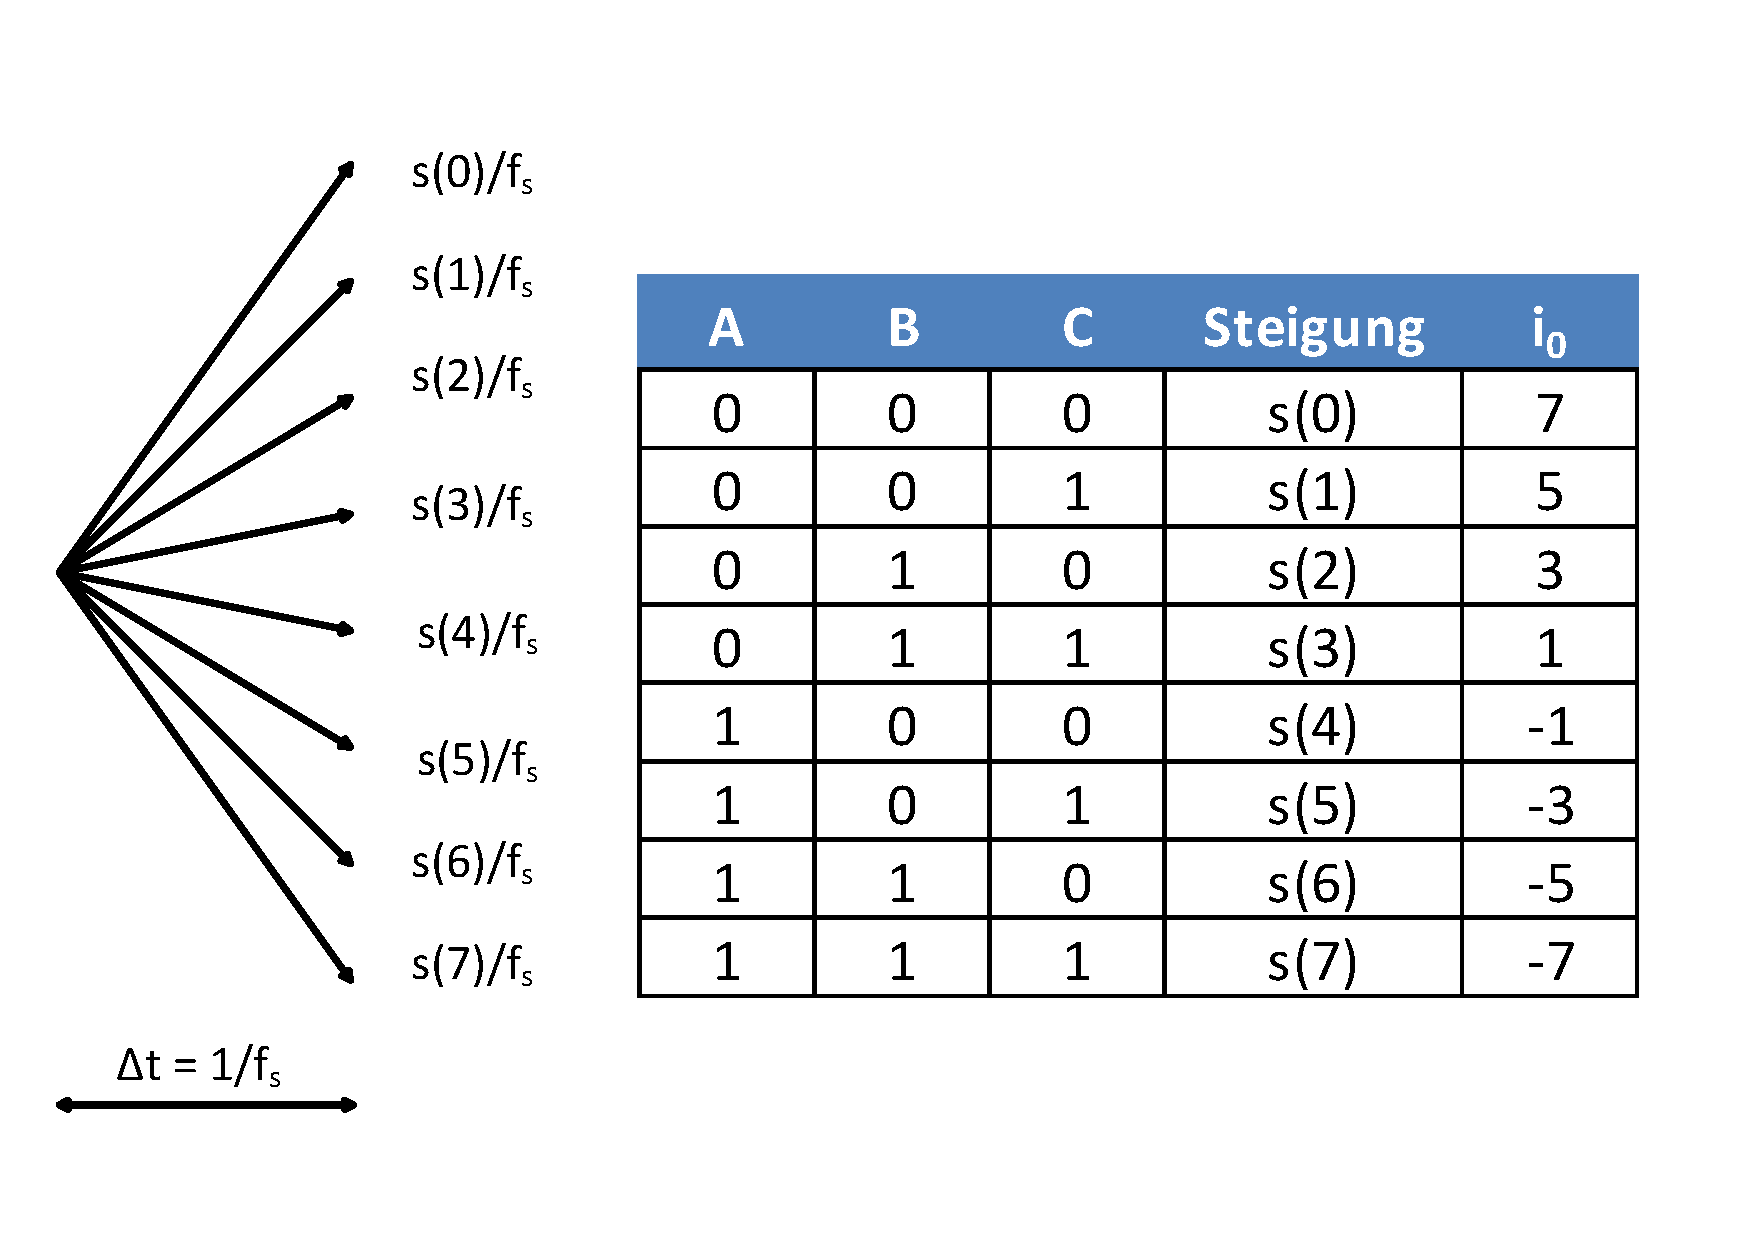
\includegraphics[width=.75\textwidth]{SlopesAndTable.pdf}
	\caption{slopes and corresponding code of the synthesized signal}
	\label{fig:SlopesAndTable}
\end{figure}

With this information a high speed digital to analog converter is created. In the following the Riemann Integral is shown.

\begin{figure}[ht]
	\centering
  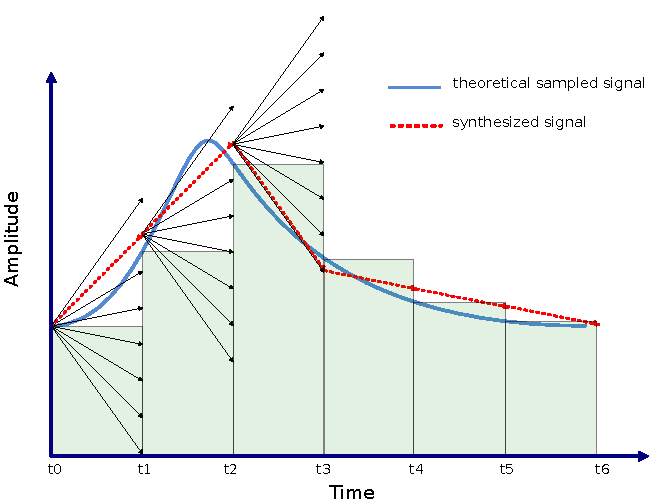
\includegraphics[width=.75\textwidth]{RiemannIntegral.pdf}
	\caption{Integral of the current which pumps charges on to the cap.}
	\label{fig:RiemannIntegral}
\end{figure}
This integral with its slopes as cited in \ref{fig:SlopesAndTable} generates the riemann code which controls the switches of the circuit. This is done by minimizing the error between the theoretical, desired signal and its synthesized one as shown in Fig. \ref{fig:RiemannIntegralError}
 \begin{figure}[ht]
	\centering
  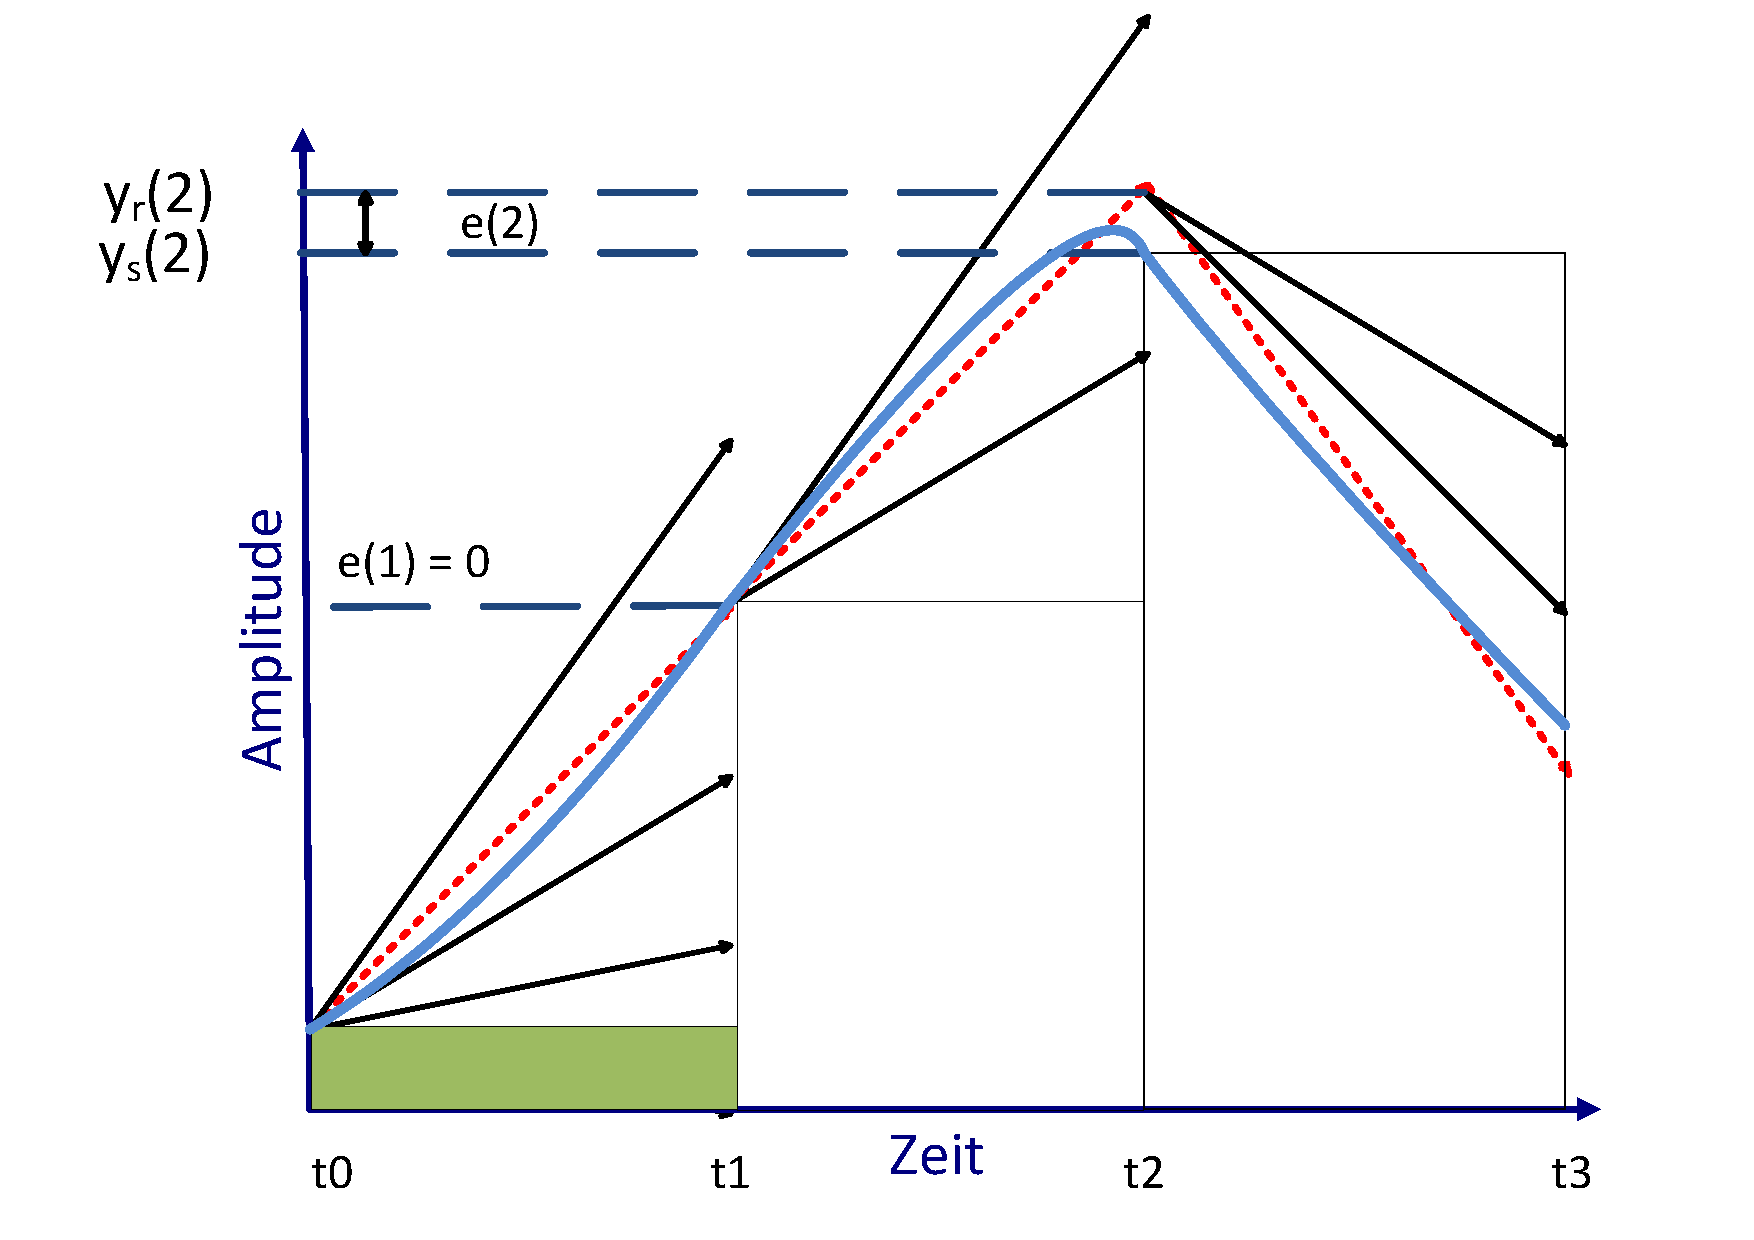
\includegraphics[width=.75\textwidth]{RiemannIntegralError.pdf}
	\caption{Code generation - error minimizing}
	\label{fig:RiemannIntegralError}
\end{figure}
The signal to noise ratio is calculated in equation \ref{eq:SNR_RiemannPumpConversion}. Quantization noise model {reference: analog device}
\begin{equation}
	\text{SNR } [\si{\dB}] = 6.02N + 9.03r - 7.78 + 10\log_{10}(1 - \frac{1}{2}^{N-1} + \frac{1}{2}^{2N})
	\label{eq:SNR_RiemannPumpConversion}
\end{equation}


%Process of the digital to analog conversion:
%\begin{enumerate}
%	\item theoretical signal generation via multiplication of time domain signals
%	\item linear approximation via error estimation to get a sequence of relative slopes
%	\item get binary code of the sequence of slopes
%	\item control switches with this digital code to synthesize the wanted analog signal
%\end{enumerate}

% \textbf{Description of the OSR, Nyquist-Shannon theorem and the SQNR...}
The \gls{ab:osr} is four and hence due to the Nyquist-Shannon theorem, the sampling \gls{sy:freq} is eight times the signal frequency.
This in mind, tuning the sampling frequency will result in tuning the signal frequency.
%\textit{introducing noise due to the conversion}
%\gls{ab:sqnr}
%The deviation of the two signals is lying in the nature of converting digital to analog in form of quantization noise.

\section{Characteristics of Digtial-to-Analog converter}
\label{ch:characteristics}
The characteristics, the performance and figure of merits are compared to classify the Riemann Pump within the conventional digital-to-analog conversion principles.
Performance: Resolution, Maximum sampling rate, dynamic range.
FOM: Gain, SFDR, SNR, settling time.\\
The characteristics of different \gls{ab:dac} is the performance and some figure of merits.
Performance leads to the generation of noise in terms of signal to (quantization) noise ratio.
This \gls{ab:sqnr} gave a good insight to the performance of the corresponding \gls{ab:dac} without to focus on energy consumption nor efficiency.
%\textit{Explain the different SNR (short), display the table to compare them.}


\section{Conclusion of the fundamentals}
In this chapter the implementation of the Riemann Pump in a system design has been presented.
After the description of the classification and application, the concept of the custom \gls{ab:dac} has been described.
After explaining a simple charge pump, a multi bit resolution \gls{ab:dac} have been presented.
The designed custom \gls{ab:dac} has been compared to conventional \gls{ab:dac} concepts.
A concise evaluation states that the Riemann Pump is a great improvement for conventional digital-to-analog conversion concepts.